\documentclass[margin=1mm]{standalone}
\usepackage[utf8]{inputenc}
\usepackage{amsmath}
\usepackage{amsfonts}
\usepackage{amssymb, bm}
\usepackage{tikz}
\usetikzlibrary{calc,arrows,positioning,shapes,shapes.gates.logic.US,trees, backgrounds}
\usetikzlibrary{decorations.pathreplacing}
\usetikzlibrary{fit, positioning}

\begin{document}
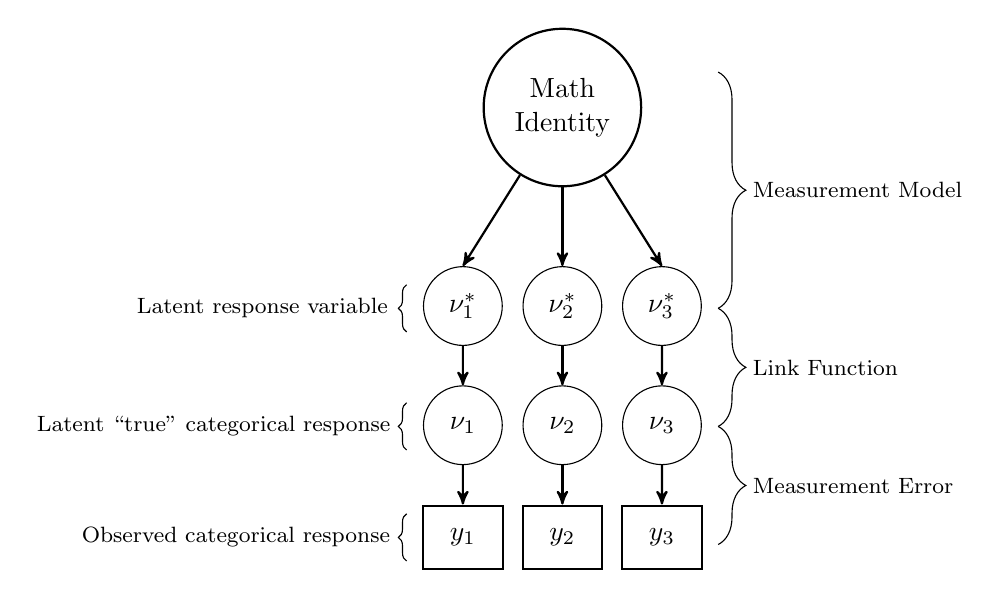
\begin{tikzpicture}[auto,scale=3,
	latent/.style={circle,draw,thick,text badly centered, inner sep=2pt,minimum size=20mm, text width=4.5em, fill=white},
	error/.style={circle,draw,text badly centered, inner sep=2pt,minimum size=10mm},
	manifest/.style={text centered, rectangle,draw,thick,inner sep=3pt,minimum height=8mm, minimum width=8mm, text width= 8 mm},
	  plate/.style={draw, shape=rectangle,thick, minimum height=4.25cm, minimum width=4.5cm, text width=1cm, align=right, inner sep=10pt, inner ysep=10pt, append after command={node[below right= 3pt of \tikzlastnode.north west] {#1}}},
	  plate2/.style={draw, shape=rectangle,thick, minimum height=4.5cm, minimum width=7cm, text width=1cm, align=right, inner sep=5pt, inner ysep=8pt, append after command={node[left= 3pt of \tikzlastnode.east] {#1}}},
	manifestRot/.style={text centered, rectangle, draw, thick,inner sep=3pt, minimum width=7mm, text width= 7mm, minimum height=15},
	manifestfront/.style={rectangle,draw,thick,inner sep=0pt,minimum size=12mm, fill=white},
	ghost/.style={rectangle, inner sep=0pt,text centered,    minimum height=0mm, minimum width=5mm, text width= 5 mm},
	lcorr/.style={<->,>=stealth', bend right=40},
	rcorr/.style={<->,>=stealth', bend left=40},
	fcorr/.style={<->,>=stealth', bend left=40},
	ofcorr/.style={<->,>=stealth', bend right=60},
	ofcorr2/.style={<->,>=stealth', bend left=60},
	intercept/.style={regular polygon,
        regular polygon sides=3,draw,thick,inner sep=0pt,minimum size=10mm},
	mean/.style={regular polygon,regular polygon sides=3,draw,thick,inner sep=0pt,minimum size=10mm},
	paths/.style={->, thick, >=stealth'},
	variance/.style={<->, thick, >=stealth', bend left=270, looseness=2},
	varianceTop/.style={<->, thick, >=stealth', bend right=270, looseness=2},
	unique/.style={<->, thick, >=stealth', loop below=270, looseness=8},
	factvar/.style={<->, thick, >=stealth', loop right=270, looseness=8}
	] % End Creating Path Model Pieces
\tikzset{mystyle/.style={->,double=black}}


% person model
\node [latent] at (0,0) (eta1) {Math Identity};
\node [error]   [below = 1cm of eta1] (lvr2) {$\nu^{\ast}_2$};
\node [error]   [left = 0.25cm of lvr2] (lvr1) {$\nu^{\ast}_1$};
\node [error]   [right = 0.25cm of lvr2] (lvr3) {$\nu^{\ast}_3$};

\node [error]   [below = 0.5cm of lvr1] (nu1) {$\nu_1$};
\node [error]   [below = 0.5cm of lvr2] (nu2) {$\nu_2$};
\node [error]   [below = 0.5cm of lvr3] (nu3) {$\nu_3$};

\node [manifest]   [below = 0.5cm of nu1] (y1) {$y_1$};
\node [manifest]   [below = 0.5cm of nu2] (y2) {$y_2$};
\node [manifest]   [below = 0.5cm of nu3] (y3) {$y_3$};

% error varaince of latent response
%\node [above left = 0.25cm of lvr1] (theta1) {$\theta_1$};
%\node [above left = 0.25cm of lvr2] (theta2) {$\theta_2$};
%\node [above left = 0.25cm of lvr3] (theta3) {$\theta_3$};
%\node [above left = 0.25cm of lvr4] (theta4) {$\theta_4$};
%\node [above left = 0.25cm of lvr5] (theta5) {$\theta_5$};

% paths
\draw[paths] (eta1)  -- (lvr1.north);
\draw[paths] (eta1)  -- (lvr2.north);
\draw[paths] (eta1)  -- (lvr3.north);

\draw[paths] (lvr1)  -- (nu1.north);
\draw[paths] (lvr2)  -- (nu2.north);
\draw[paths] (lvr3)  -- (nu3.north);

\draw[paths] (nu1)  -- (y1.north);
\draw[paths] (nu2)  -- (y2.north);
\draw[paths] (nu3)  -- (y3.north);

%\draw[paths] (theta1)  -- (lvr1);
%\draw[paths] (theta2)  -- (lvr2);
%\draw[paths] (theta3)  -- (lvr3);
%\draw[paths] (theta4)  -- (lvr4);
%\draw[paths] (theta5)  -- (lvr5);

% build braces for pieces of the model
\draw [decorate,decoration={brace,amplitude=10pt},xshift=-4pt,yshift=0pt] (0.8,0.15) -- (0.8,-0.85) node [black,midway,xshift=9pt] {\footnotesize Measurement Model};
\draw [decorate,decoration={brace,amplitude=10pt},xshift=-4pt,yshift=0pt] (0.8,-0.85) -- (0.8,-1.35) node [black,midway,xshift=9pt] {\footnotesize Link Function};
\draw [decorate,decoration={brace,amplitude=10pt},xshift=-4pt,yshift=0pt] (0.8,-1.35) -- (0.8,-1.85) node [black,midway,xshift=9pt] {\footnotesize Measurement Error};

\draw [decorate,decoration={brace,amplitude=3pt, mirror},xshift=4pt,yshift=0pt] (-0.8,-0.75) -- (-0.8,-0.95) node [black,midway,xshift=-3.55cm] {\footnotesize Latent response variable}; 
\draw [decorate,decoration={brace,amplitude=3pt, mirror},xshift=4pt,yshift=0pt] (-0.8,-1.25) -- (-0.8,-1.45) node [black,midway,xshift=-4.82cm]{\footnotesize Latent ``true'' categorical response};
\draw [decorate,decoration={brace,amplitude=3pt, mirror},xshift=4pt,yshift=0pt] (-0.8,-1.72) -- (-0.8,-1.92) node [black,midway,xshift=-4.25cm] {\footnotesize Observed categorical response};

\end{tikzpicture}
\end{document}